\documentclass[tikz,border=12pt]{standalone}
\usepackage[T1]{fontenc}
\usepackage{mathpazo}
\usepackage{amsmath,amssymb}
\usetikzlibrary{arrows.meta, positioning, calc, fit, decorations.pathreplacing, patterns}

\definecolor{stblue}{HTML}{7B97AD}
\definecolor{rwgold}{HTML}{B8995E}
\definecolor{sage}{HTML}{7A9A7E}
\definecolor{dkbrown}{HTML}{3D3530}
\definecolor{wmgray}{HTML}{7B7067}
\definecolor{cream}{HTML}{F9F6F0}
\definecolor{border}{HTML}{D4C9B8}
\definecolor{terracotta}{HTML}{C47A6A}
\definecolor{lavender}{HTML}{907EA0}

\begin{document}
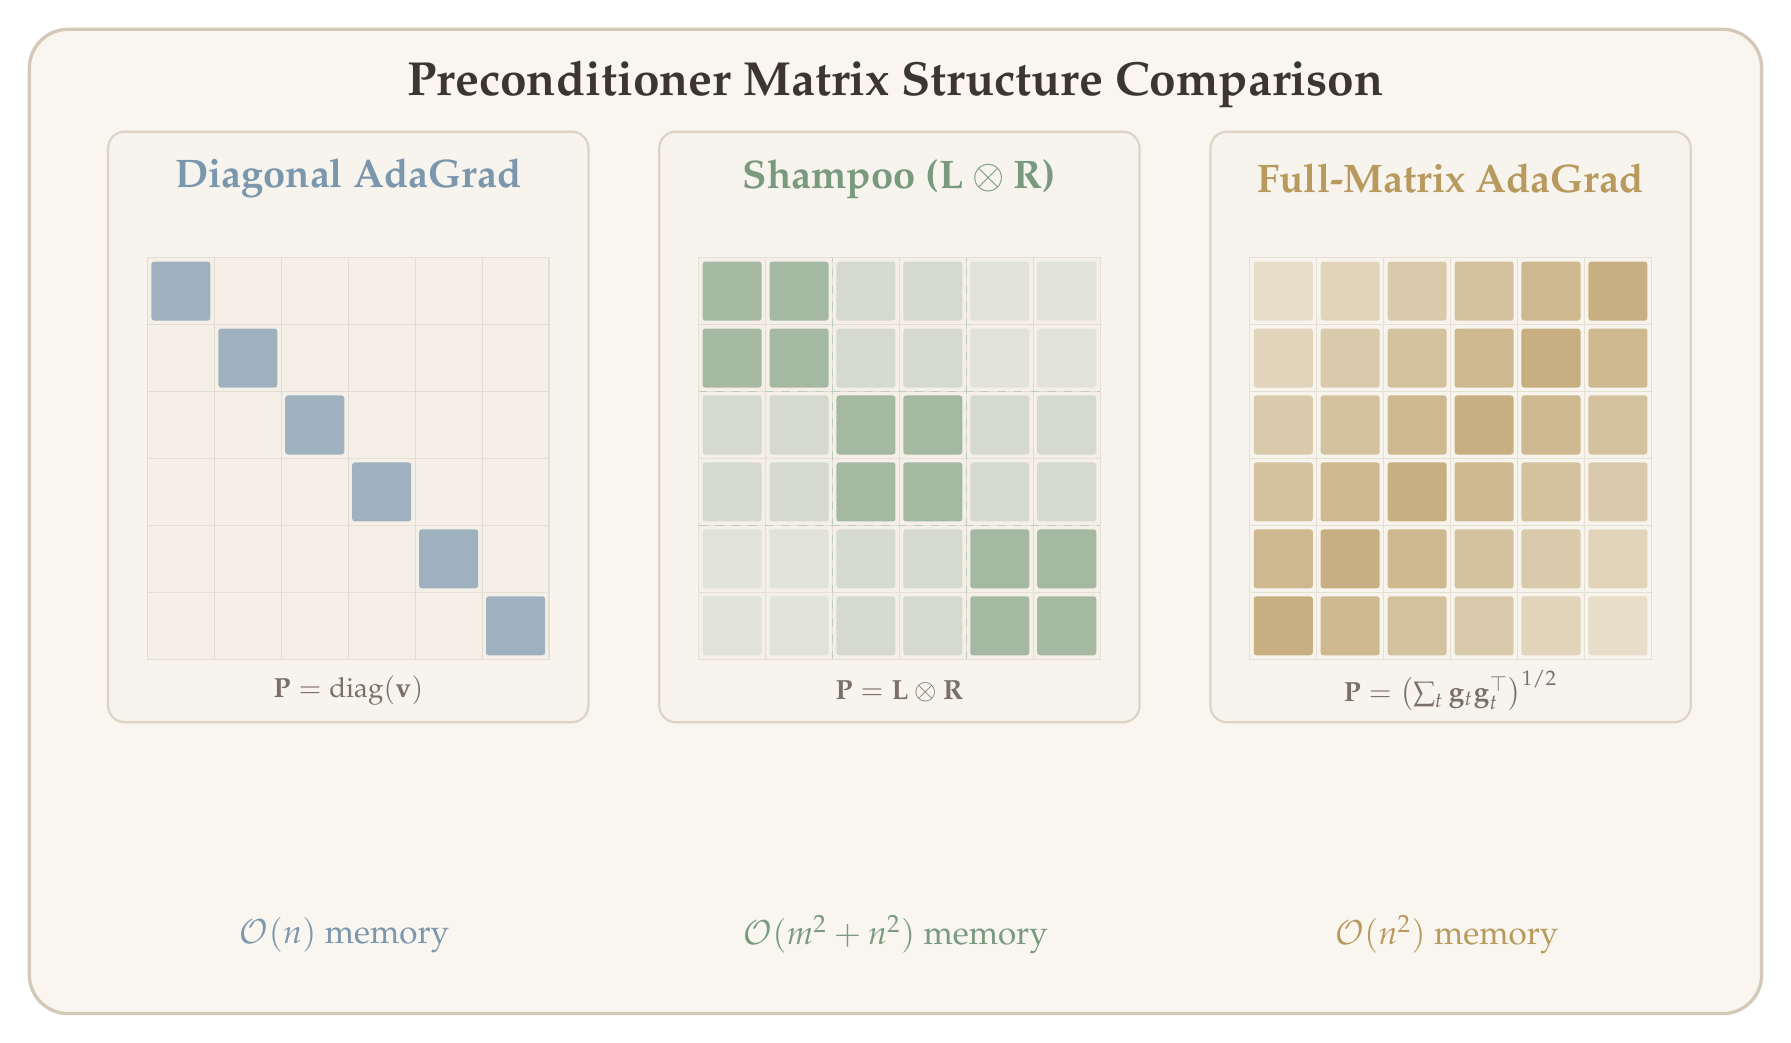
\begin{tikzpicture}[>={Stealth[length=4mm, width=3mm]}, line width=1.5pt]

% Background
\fill[cream, rounded corners=14pt] (-0.5,-3.0) rectangle (21.5,9.5);
\draw[border, line width=1.2pt, rounded corners=14pt] (-0.5,-3.0) rectangle (21.5,9.5);

% Title
\node[text=dkbrown, font=\LARGE\bfseries] at (10.5,8.8) {Preconditioner Matrix Structure Comparison};

\def\cellsize{0.85}
\def\gridsize{6}

% ============================================================
% Panel 1: Diagonal AdaGrad
% ============================================================
\def\pAx{1.0}
\def\pAy{1.5}

% Panel background
\fill[cream!95!border, rounded corners=6pt] ($({\pAx-0.5},{\pAy-0.8})$) rectangle ($({\pAx+\gridsize*\cellsize+0.5},{\pAy+\gridsize*\cellsize+1.6})$);
\draw[border!80, line width=0.8pt, rounded corners=6pt] ($({\pAx-0.5},{\pAy-0.8})$) rectangle ($({\pAx+\gridsize*\cellsize+0.5},{\pAy+\gridsize*\cellsize+1.6})$);

% Panel title
\node[text=stblue, font=\Large\bfseries] at ($({\pAx+\gridsize*\cellsize/2},{\pAy+\gridsize*\cellsize+1.0})$) {Diagonal AdaGrad};

% Grid
\foreach \i in {0,...,5} {
  \foreach \j in {0,...,5} {
    % Empty cell
    \draw[border!60, line width=0.4pt]
      ($({\pAx+\j*\cellsize},{\pAy+\i*\cellsize})$)
      rectangle
      ($({\pAx+\j*\cellsize+\cellsize},{\pAy+\i*\cellsize+\cellsize})$);
    \fill[border, opacity=0.08]
      ($({\pAx+\j*\cellsize},{\pAy+\i*\cellsize})$)
      rectangle
      ($({\pAx+\j*\cellsize+\cellsize},{\pAy+\i*\cellsize+\cellsize})$);
  }
}

% Diagonal cells filled (i==j, but row 0 is bottom)
\foreach \k in {0,...,5} {
  \pgfmathsetmacro{\ri}{5-\k} % flip so row 0 = top visually
  \fill[stblue, opacity=0.7, rounded corners=1pt]
    ($({\pAx+\k*\cellsize+0.05},{\pAy+\ri*\cellsize+0.05})$)
    rectangle
    ($({\pAx+\k*\cellsize+\cellsize-0.05},{\pAy+\ri*\cellsize+\cellsize-0.05})$);
}

% Label
\node[text=wmgray, font=\normalsize\itshape] at ($({\pAx+\gridsize*\cellsize/2},{\pAy-0.4})$) {$\mathbf{P} = \mathrm{diag}(\mathbf{v})$};

% ============================================================
% Panel 2: Shampoo (L x R)
% ============================================================
\def\pBx{8.0}
\def\pBy{1.5}

% Panel background
\fill[cream!95!border, rounded corners=6pt] ($({\pBx-0.5},{\pBy-0.8})$) rectangle ($({\pBx+\gridsize*\cellsize+0.5},{\pBy+\gridsize*\cellsize+1.6})$);
\draw[border!80, line width=0.8pt, rounded corners=6pt] ($({\pBx-0.5},{\pBy-0.8})$) rectangle ($({\pBx+\gridsize*\cellsize+0.5},{\pBy+\gridsize*\cellsize+1.6})$);

% Panel title
\node[text=sage, font=\Large\bfseries] at ($({\pBx+\gridsize*\cellsize/2},{\pBy+\gridsize*\cellsize+1.0})$) {Shampoo ($\mathbf{L} \otimes \mathbf{R}$)};

% Grid with Kronecker block pattern
% Shampoo uses L (kron) R structure: 3x3 blocks of 2x2
\foreach \i in {0,...,5} {
  \foreach \j in {0,...,5} {
    \draw[border!60, line width=0.4pt]
      ($({\pBx+\j*\cellsize},{\pBy+\i*\cellsize})$)
      rectangle
      ($({\pBx+\j*\cellsize+\cellsize},{\pBy+\i*\cellsize+\cellsize})$);
    \fill[border, opacity=0.08]
      ($({\pBx+\j*\cellsize},{\pBy+\i*\cellsize})$)
      rectangle
      ($({\pBx+\j*\cellsize+\cellsize},{\pBy+\i*\cellsize+\cellsize})$);
  }
}

% Fill Kronecker block pattern: 3 blocks of 2x2 along diagonal, plus cross-block coupling
% Block (0,0): rows 4-5, cols 0-1
% Block (1,1): rows 2-3, cols 2-3
% Block (2,2): rows 0-1, cols 4-5
% Also partial fill for off-diagonal blocks with lower opacity
\foreach \br/\bc in {0/0, 0/1, 1/0, 1/1} {
  % Block (0,0) at top-left
  \pgfmathsetmacro{\ri}{5-\br}
  \pgfmathsetmacro{\cj}{\bc}
  \fill[sage, opacity=0.65, rounded corners=1pt]
    ($({\pBx+\cj*\cellsize+0.05},{\pBy+\ri*\cellsize+0.05})$)
    rectangle
    ($({\pBx+\cj*\cellsize+\cellsize-0.05},{\pBy+\ri*\cellsize+\cellsize-0.05})$);
  % Block (1,1) in middle
  \pgfmathsetmacro{\ri}{5-(\br+2)}
  \pgfmathsetmacro{\cj}{\bc+2}
  \fill[sage, opacity=0.65, rounded corners=1pt]
    ($({\pBx+\cj*\cellsize+0.05},{\pBy+\ri*\cellsize+0.05})$)
    rectangle
    ($({\pBx+\cj*\cellsize+\cellsize-0.05},{\pBy+\ri*\cellsize+\cellsize-0.05})$);
  % Block (2,2) at bottom-right
  \pgfmathsetmacro{\ri}{5-(\br+4)}
  \pgfmathsetmacro{\cj}{\bc+4}
  \fill[sage, opacity=0.65, rounded corners=1pt]
    ($({\pBx+\cj*\cellsize+0.05},{\pBy+\ri*\cellsize+0.05})$)
    rectangle
    ($({\pBx+\cj*\cellsize+\cellsize-0.05},{\pBy+\ri*\cellsize+\cellsize-0.05})$);
}

% Off-diagonal blocks with lower opacity
\foreach \br/\bc in {0/0, 0/1, 1/0, 1/1} {
  % Block (0,1): rows 4-5, cols 2-3
  \pgfmathsetmacro{\ri}{5-\br}
  \pgfmathsetmacro{\cj}{\bc+2}
  \fill[sage, opacity=0.25, rounded corners=1pt]
    ($({\pBx+\cj*\cellsize+0.05},{\pBy+\ri*\cellsize+0.05})$)
    rectangle
    ($({\pBx+\cj*\cellsize+\cellsize-0.05},{\pBy+\ri*\cellsize+\cellsize-0.05})$);
  % Block (1,0): rows 2-3, cols 0-1
  \pgfmathsetmacro{\ri}{5-(\br+2)}
  \pgfmathsetmacro{\cj}{\bc}
  \fill[sage, opacity=0.25, rounded corners=1pt]
    ($({\pBx+\cj*\cellsize+0.05},{\pBy+\ri*\cellsize+0.05})$)
    rectangle
    ($({\pBx+\cj*\cellsize+\cellsize-0.05},{\pBy+\ri*\cellsize+\cellsize-0.05})$);
  % Block (0,2): rows 4-5, cols 4-5
  \pgfmathsetmacro{\ri}{5-\br}
  \pgfmathsetmacro{\cj}{\bc+4}
  \fill[sage, opacity=0.15, rounded corners=1pt]
    ($({\pBx+\cj*\cellsize+0.05},{\pBy+\ri*\cellsize+0.05})$)
    rectangle
    ($({\pBx+\cj*\cellsize+\cellsize-0.05},{\pBy+\ri*\cellsize+\cellsize-0.05})$);
  % Block (2,0): rows 0-1, cols 0-1
  \pgfmathsetmacro{\ri}{5-(\br+4)}
  \pgfmathsetmacro{\cj}{\bc}
  \fill[sage, opacity=0.15, rounded corners=1pt]
    ($({\pBx+\cj*\cellsize+0.05},{\pBy+\ri*\cellsize+0.05})$)
    rectangle
    ($({\pBx+\cj*\cellsize+\cellsize-0.05},{\pBy+\ri*\cellsize+\cellsize-0.05})$);
  % Block (1,2): rows 2-3, cols 4-5
  \pgfmathsetmacro{\ri}{5-(\br+2)}
  \pgfmathsetmacro{\cj}{\bc+4}
  \fill[sage, opacity=0.25, rounded corners=1pt]
    ($({\pBx+\cj*\cellsize+0.05},{\pBy+\ri*\cellsize+0.05})$)
    rectangle
    ($({\pBx+\cj*\cellsize+\cellsize-0.05},{\pBy+\ri*\cellsize+\cellsize-0.05})$);
  % Block (2,1): rows 0-1, cols 2-3
  \pgfmathsetmacro{\ri}{5-(\br+4)}
  \pgfmathsetmacro{\cj}{\bc+2}
  \fill[sage, opacity=0.25, rounded corners=1pt]
    ($({\pBx+\cj*\cellsize+0.05},{\pBy+\ri*\cellsize+0.05})$)
    rectangle
    ($({\pBx+\cj*\cellsize+\cellsize-0.05},{\pBy+\ri*\cellsize+\cellsize-0.05})$);
}

% Block boundary lines
\foreach \k in {2,4} {
  \draw[sage!50, line width=0.6pt, dashed]
    ($({\pBx+\k*\cellsize},{\pBy})$) -- ($({\pBx+\k*\cellsize},{\pBy+\gridsize*\cellsize})$);
  \pgfmathsetmacro{\ri}{\gridsize-\k}
  \draw[sage!50, line width=0.6pt, dashed]
    ($({\pBx},{\pBy+\k*\cellsize})$) -- ($({\pBx+\gridsize*\cellsize},{\pBy+\k*\cellsize})$);
}

% Label
\node[text=wmgray, font=\normalsize\itshape] at ($({\pBx+\gridsize*\cellsize/2},{\pBy-0.4})$) {$\mathbf{P} = \mathbf{L} \otimes \mathbf{R}$};

% ============================================================
% Panel 3: Full-Matrix AdaGrad
% ============================================================
\def\pCx{15.0}
\def\pCy{1.5}

% Panel background
\fill[cream!95!border, rounded corners=6pt] ($({\pCx-0.5},{\pCy-0.8})$) rectangle ($({\pCx+\gridsize*\cellsize+0.5},{\pCy+\gridsize*\cellsize+1.6})$);
\draw[border!80, line width=0.8pt, rounded corners=6pt] ($({\pCx-0.5},{\pCy-0.8})$) rectangle ($({\pCx+\gridsize*\cellsize+0.5},{\pCy+\gridsize*\cellsize+1.6})$);

% Panel title
\node[text=rwgold, font=\Large\bfseries] at ($({\pCx+\gridsize*\cellsize/2},{\pCy+\gridsize*\cellsize+1.0})$) {Full-Matrix AdaGrad};

% Grid - fully filled with varying opacity
\foreach \i in {0,...,5} {
  \foreach \j in {0,...,5} {
    \draw[border!60, line width=0.4pt]
      ($({\pCx+\j*\cellsize},{\pCy+\i*\cellsize})$)
      rectangle
      ($({\pCx+\j*\cellsize+\cellsize},{\pCy+\i*\cellsize+\cellsize})$);
    % Opacity based on distance from diagonal
    \pgfmathsetmacro{\dist}{abs(\i-\j)}
    \pgfmathsetmacro{\opac}{0.75 - \dist*0.1}
    \fill[rwgold, opacity=\opac, rounded corners=1pt]
      ($({\pCx+\j*\cellsize+0.05},{\pCy+\i*\cellsize+0.05})$)
      rectangle
      ($({\pCx+\j*\cellsize+\cellsize-0.05},{\pCy+\i*\cellsize+\cellsize-0.05})$);
  }
}

% Label
\node[text=wmgray, font=\normalsize\itshape] at ($({\pCx+\gridsize*\cellsize/2},{\pCy-0.4})$) {$\mathbf{P} = \bigl(\sum_t \mathbf{g}_t \mathbf{g}_t^\top\bigr)^{1/2}$};

% ============================================================
% Bottom annotations
% ============================================================
\node[text=stblue, font=\large] at (3.5,-2.0) {$\mathcal{O}(n)$ memory};
\node[text=sage, font=\large] at (10.5,-2.0) {$\mathcal{O}(m^2 + n^2)$ memory};
\node[text=rwgold, font=\large] at (17.5,-2.0) {$\mathcal{O}(n^2)$ memory};

\end{tikzpicture}
\end{document}
